\documentclass[11pt, a4paper]{article}

% --- Paquetes esenciales ---
\usepackage[utf8]{inputenc}
\usepackage[spanish, es-tabla]{babel}
\usepackage[top=3cm, bottom=2.5cm, left=2.5cm, right=2.5cm]{geometry}
\usepackage{graphicx}
\usepackage{xcolor}
\usepackage{fancyhdr}
\usepackage{titlesec}
\usepackage{booktabs}
\usepackage{float}
\usepackage{hyperref}
\usepackage{fontspec}
\setmainfont{Poppins} % Llama a la tipografia Poppins nativa de Windows

% --- Paleta Corporativa Fintual ---
\definecolor{FintualLightBlue}{HTML}{9FCDFF}
\definecolor{FintualBlue}{HTML}{005AE6}
\definecolor{FintualDarkBlue}{HTML}{003295}
\definecolor{FintualDark}{HTML}{22262F}

\hypersetup{
    colorlinks=true,
    linkcolor=FintualBlue,
    urlcolor=FintualBlue
}

% --- Configuracion de Header y Footer ---
\pagestyle{fancy}
\fancyhf{}
\setlength{\headheight}{35pt}
\fancyhead[L]{
\includegraphics[width=3cm]{logo.jpg}}
\fancyhead[R]{\textcolor{FintualDark}{\small Módulo de Gestión de Portafolios}}
\fancyfoot[C]{\thepage}
\renewcommand{\headrulewidth}{0.8pt}
\renewcommand{\headrule}{\hbox to\headwidth{\color{FintualLightBlue}\leaders\hrule height \headrulewidth\hfill}}

% Estilo de titulos
\titleformat{\section}{\Large\bfseries\color{FintualDarkBlue}}{\thesection}{1em}{}
\titleformat{\subsection}{\large\bfseries\color{FintualBlue}}{\thesubsection}{1em}{}

\begin{document}

% --- Metadatos ---
\noindent
\textbf{Módulo de Gestión de Portafolios} \\
\textbf{Autor:} Ronald Leblebici Garo \\
\textbf{Fecha:} \today \\
\vspace{0.5cm}

\section{Resumen Ejecutivo}

\textbf{Objetivo:} Este reporte documenta el diseño y la implementación de un módulo de gestión de portafolio que podría constituir parte de una aplicación de inversión y trading personal en la vida real. Según las indicaciones, se creó una clase ``Portfolio'' que recibe los datos de precios diarios de los activos que se pretenden mantener en los portafolios seleccionados. Además, se diseñó un método para calibrar las diferentes carteras, estableciendo qué activo comprar o vender cada mes y en qué medida. Este documento sintetiza el proceso, implementación, razonamiento y resultados del trabajo realizado. \\

\textbf{Datos:} Se extrajeron datos de activos financieros desde la \href{https://fintual.cl/api-docs/index.html}{API de Fintual} y del S\&P500 disponibles en Yahoo Finance, con el objetivo de acotar el universo a valores que realmente se puedan transar en una app como la de Fintual. En lo temporal, distinguimos dos períodos: el de ``observación'' (mayo/23 - mayo/25)y el de ``prueba'' (mayo/25 - mayo/26). \\

\textbf{Metodología:} Los portafolios fueron diseñados usando CAPM, aunque se introdujo un tope máximo de 15\% de participación de cada activo en un mismo portafolio y objetivos de $\beta$ de mercado. En el período de prueba se hicieron los rebalanceos correspondientes a cada portafolio al final de cada mes. Por simplicidad, nuestra regla de balanceo periódico no establece umbrales a partir de los cuales haya que comprar o vender. Simplemente se calculan las brechas entre la asignación porcentual vigente y objetivo para cada activo en cada portafolio. Los que están sobreponderados son vendidos para comprar más de los subponderados en la medida de que el cálculo actualizado lo requiera para mantener el balance establecido vía CAPM. \\

\textbf{Resultados:} Se obtuvo portafolios eficientes, en los que se puede invertir en el mundo real y respaldadas por backtesting en el sentido de meximizar la relación entre retorno y riesgo. Los retornos anualizados fluctúan entre un 19,5 \% y un 88,8 \%, los drawdowns máximos entre un -8,3 \% y un -15,9 \% y los ratios de Sharpe entre un 2,17 y un 3,28. Esto muestra que estamos ante portafolios bien definidos, pero con perfiles de riesgos muy distintos. Todas compensan el riesgo que toman, siendo la diferencia el retorno extra que se obtiene a costa de más volatilidad y caídas.  Esto último se puede concluir a partir de los ratios de Sharpe relativamente altos. El portafolio agresivo es el más eficiente en compensar riesgo a través del retorno, aunque es el que tolera el mayor drawdown. \\

Simulando la situación de alguien que invierte 10.000 USD durante el período de prueba, en un año este habría obtenido 11{.}938{,}8 en caso de escoger el portafolio conservador, 13{.}051{,}3 en el caso moderado y 18{.}834{,}6 USD en el caso agresivo.

\section{Desempeño y Validación Teórica}

\subsection{CAPM y FPP}

Las figuras \ref{fig:grafico-capm-frontera} y \ref{fig:fpp} muestran el resultado de graficar elementos del modelo de valoración de activos de capital (CAPM) y la frontera de posibilidades de portafolio (FPP) respectivamente. Mientras el primer gráfico nos muestra que los portafolios diseñados se encuentran sobre la capital market line (siendo eficiente en términos de riesgo y retorno), el segundo nos muestra que el modelo de asignación fue exitoso. En este último se ve claramente que el portafolio moderado se ajusta a la frontera eficiente. Por su parte, el portafolio asume un rol maximizador ubicándose en la parte superior derecha y el conservador parece estar en un nivel óptimo ``a la defensiva''.

\begin{figure}[H]
    \centering
    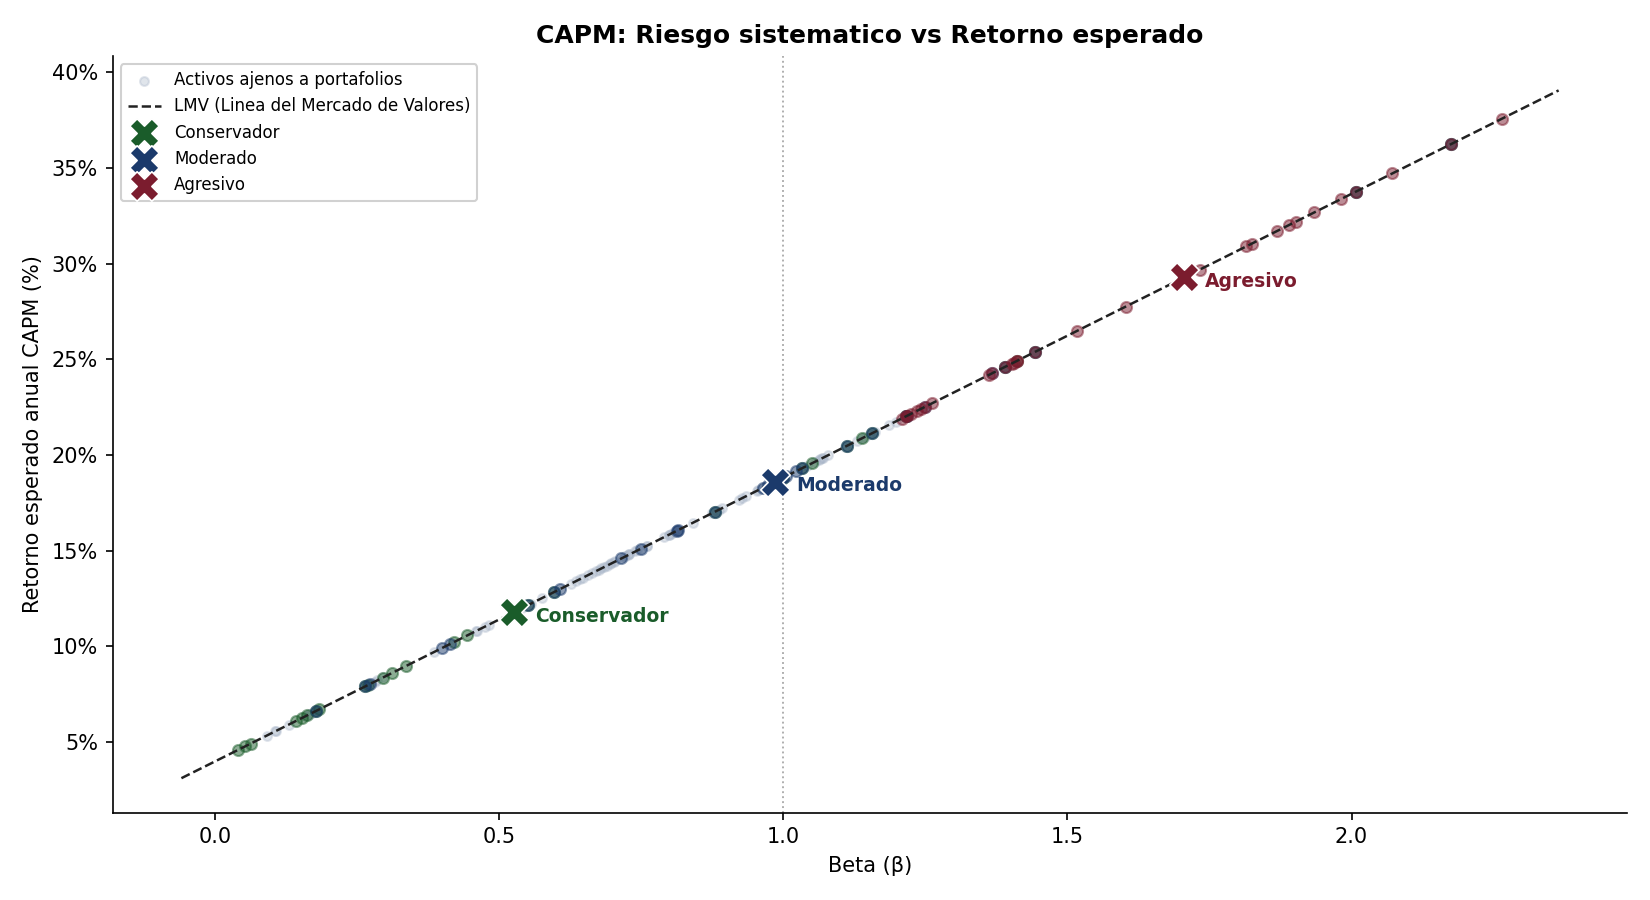
\includegraphics[width=0.85\textwidth]{../output/grafico-capm-frontera.png}
    \caption{Frontera de Posibilidades de Portafolio (FPP) y perfiles simulados.}
    \label{fig:grafico-capm-frontera}
\end{figure}

\begin{figure}[H]
    \centering
    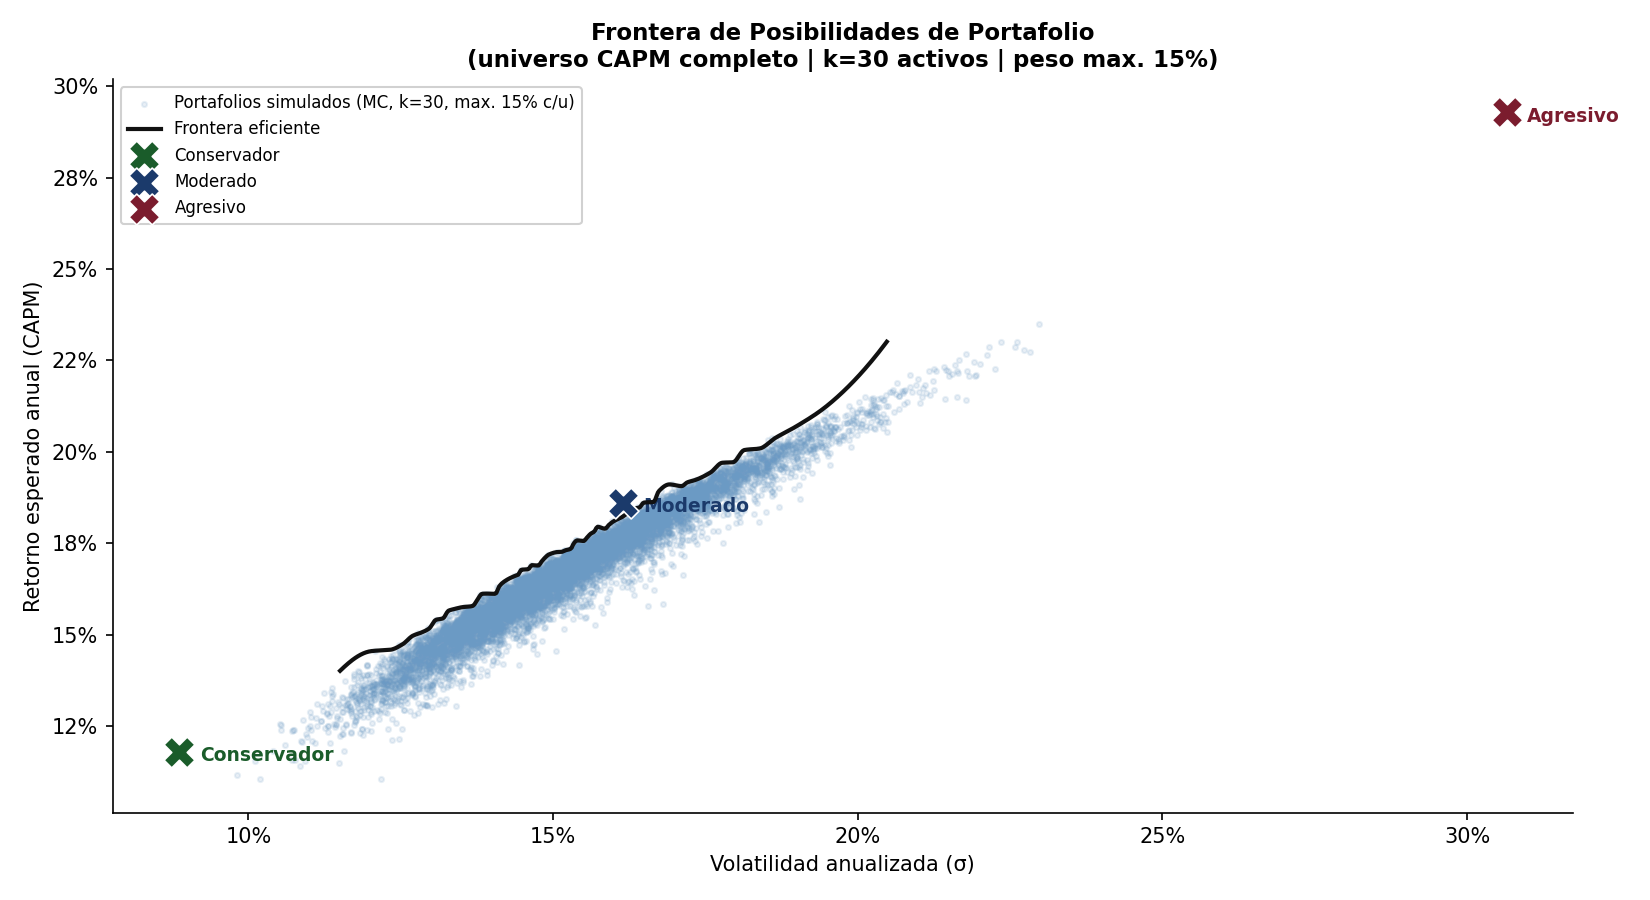
\includegraphics[width=0.85\textwidth]{../output/grafico-fpp.png}
    \caption{Frontera de Posibilidades de Portafolio (FPP) y perfiles simulados.}
    \label{fig:fpp}
\end{figure}

\subsection{Métricas y Drawdown}

Como se mencionó anteriormente, el portafolio agresivo muestra un retorno mucho mayor al del conservador ($ 88.82 \% / 19.47 \% = 4.56 $ veces), pero esto habría significado para los inversionistas soportar un drawdown de casi un 16\% en periodos de contracción (como ocurrió en abril de 2026). 

\begin{figure}[H]
    \centering
    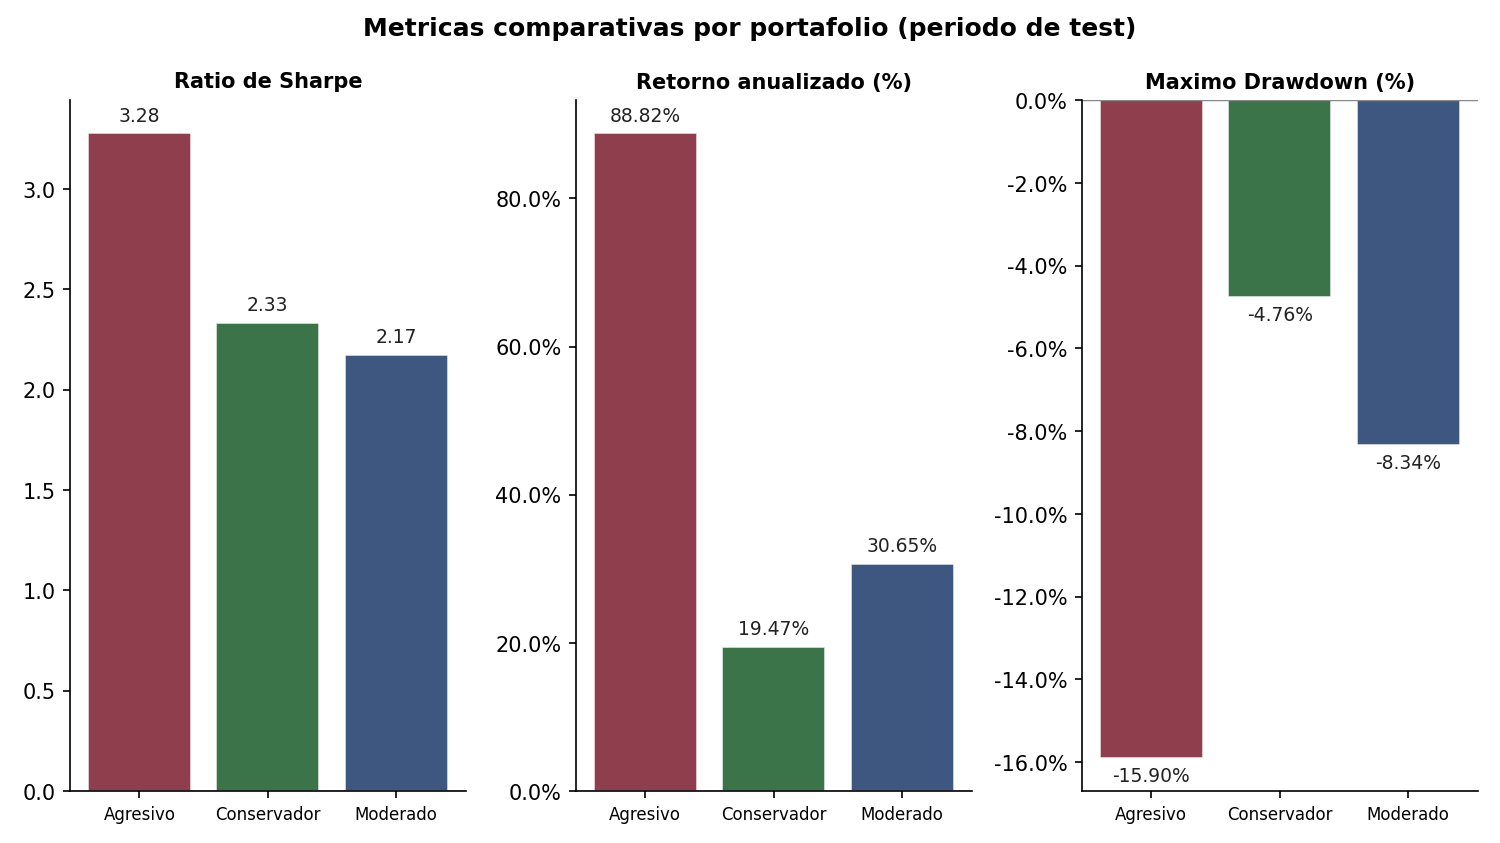
\includegraphics[width=0.9\textwidth]{../output/grafico-metricas-comparativas.png}
    \caption{Métricas comparativas (Sharpe, Retorno Anualizado y Max Drawdown).}
    \label{fig:metricas}
\end{figure}

\begin{figure}[H]
    \centering
    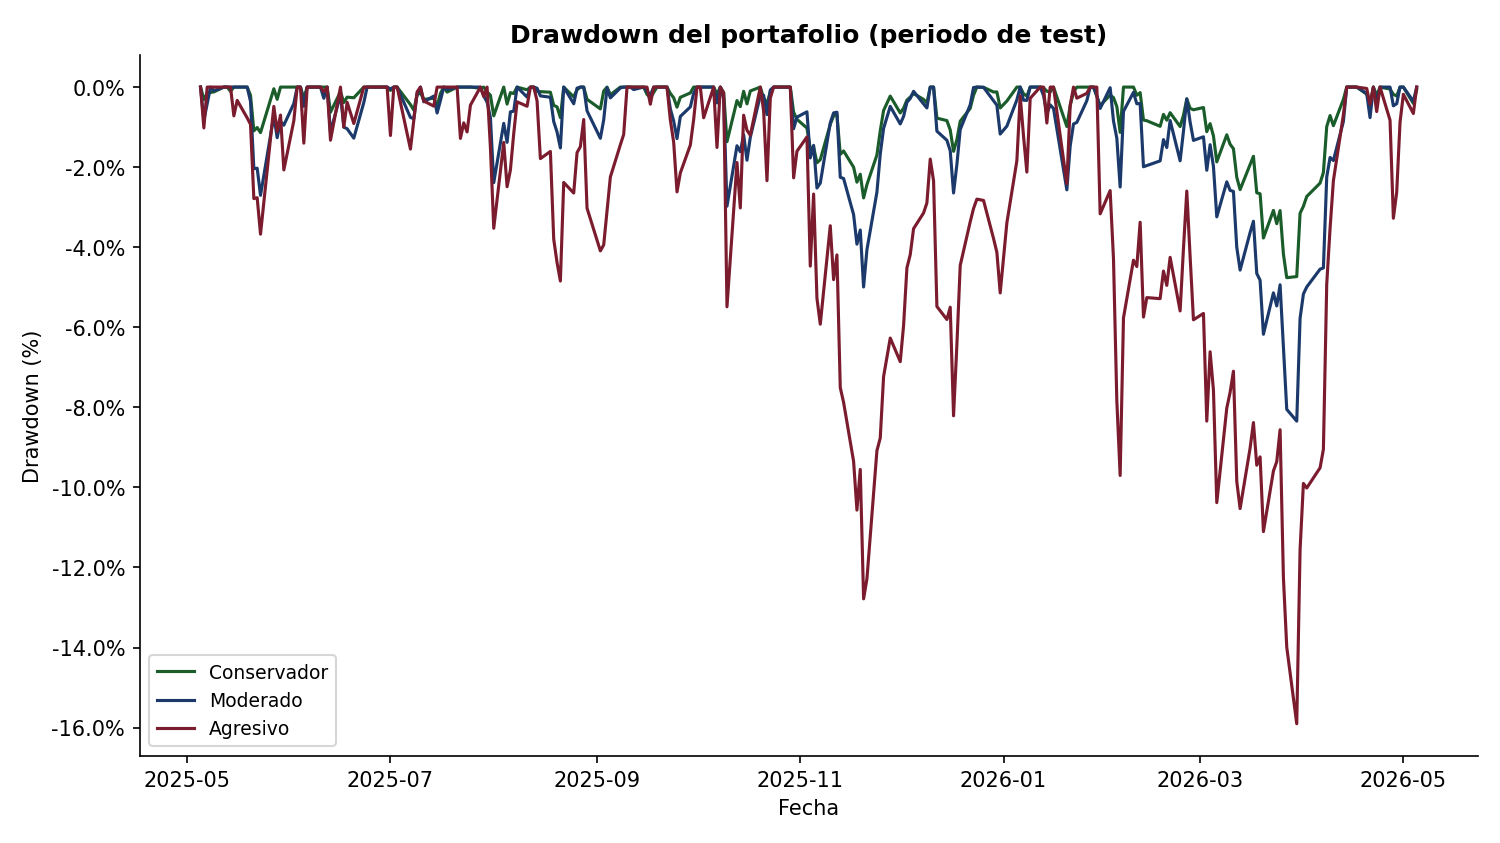
\includegraphics[width=0.85\textwidth]{../output/grafico-drawdown.png}
    \caption{Caídas máximas desde el pico (\textit{Drawdown}) por perfil.}
    \label{fig:drawdown}
\end{figure}

La evolución del valor neto de los activos (NAV) evidencia que la construcción teórica se sostiene en la práctica: el perfil moderado sigue estrechamente al activo representativo del mercado (SPY), y los extremos cumplen sus respectivas funciones.

\begin{figure}[H]
    \centering
    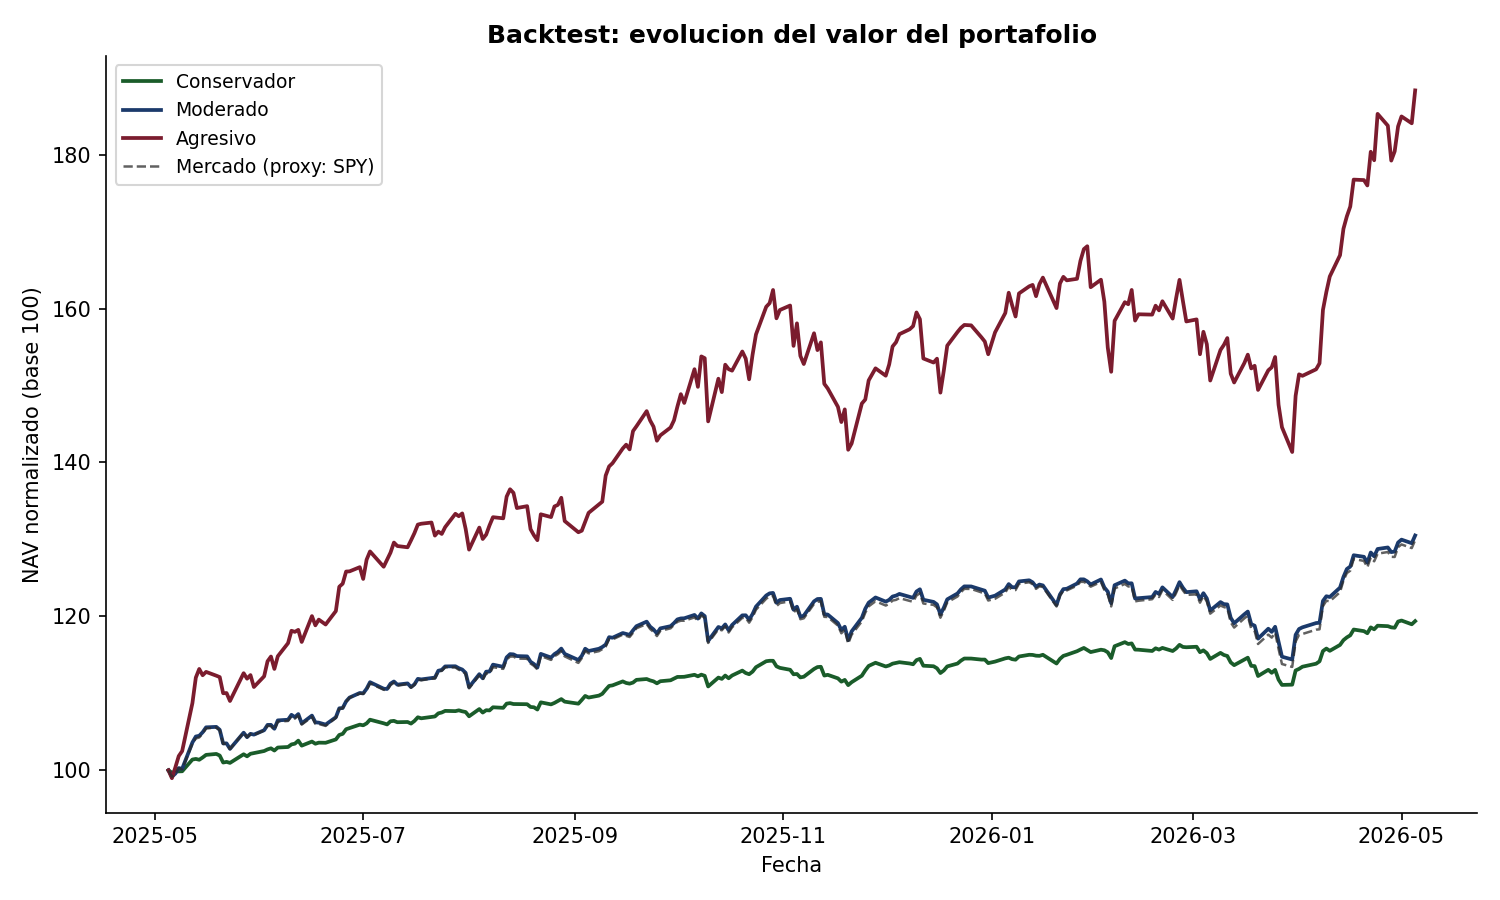
\includegraphics[width=0.85\textwidth]{../output/grafico-backtest-nav.png}
    \caption{Evolución del NAV normalizado de los portafolios frente al mercado.}
    \label{fig:backtest_nav}
\end{figure}


\section{Algoritmo de Rebalanceo (Propuesta Técnica)}

El desafío propuesto consiste en implementar un método en la clase \texttt{Portfolio} para establecer qué activos comprar y vender para llevar la cartera real hacia la asignación teórica.

\subsection{Lógica de Ejecución (Implementación Actual)}
En este ejercicio se utiliza un rebalanceo determinista forzoso: 
\begin{enumerate}
    \item Se calcula la valoración vigente de cada activo poseído en cada portafolio.
    \item Se calcula el NAV total del fondo.
    \item Se contrasta el peso real de cada activo contra el porcentaje objetivo.
    \item Se calculan las ventas de activos excedentes y las compras de faltantes.
\end{enumerate}

\subsection{Consideración de costos operativos}

Es importante tener en consideración una limitación de este ejercicio. Rebalancear constantemente el 100\% de las carteras incrementa los costos operativos. Una forma de resolver este asunto es añadir un grado de tolerancia. Por ejemplo, comprar o vender solo si el el peso de un activo se desvía más de un 3\% en magnitud de su objetivo (ya sea por sobre o subponderación).

\newpage

\section{Anexo: Detalles de Optimización y Composición}

Este anexo recopila el detalle exhaustivo del proceso de optimización, el resumen cuantitativo del backtest por portafolio, y el \textit{allocation} resultante que es consumido por la clase de rebalanceo de órdenes.

\subsection{Resumen Global del Backtest}
\begin{table}[htbp]
\centering
\begin{tabular}{lrrrrrrr}
\hline
Portafolio & $NAV_{inicio}$ & $NAV_{fin}$ & $R_{total}$ & $R_{anual}$ & Vol. anual & Sharpe & Max Drawdown \\
\hline
Agresivo & 10,000.0 & 18,834.6 & 0.88 & 0.89 & 0.26 & 3.28 & -0.16 \\
Conservador & 10,000.0 & 11,938.8 & 0.19 & 0.19 & 0.06 & 2.33 & -0.05 \\
Moderado & 10,000.0 & 13,051.4 & 0.31 & 0.31 & 0.12 & 2.17 & -0.08 \\
\hline
\end{tabular}
\caption{Resumen backtest portafolios}
\label{tab:backtest-resumen}
\end{table}

\subsection{Perfil Agresivo}
El portafolio agresivo destina el límite del 15\% permitido por activo a concentrarse agresivamente en instrumentos de semiconductores y tecnología de punta (TSLA, NVDA, AMD).

\begin{figure}[H]
    \centering
    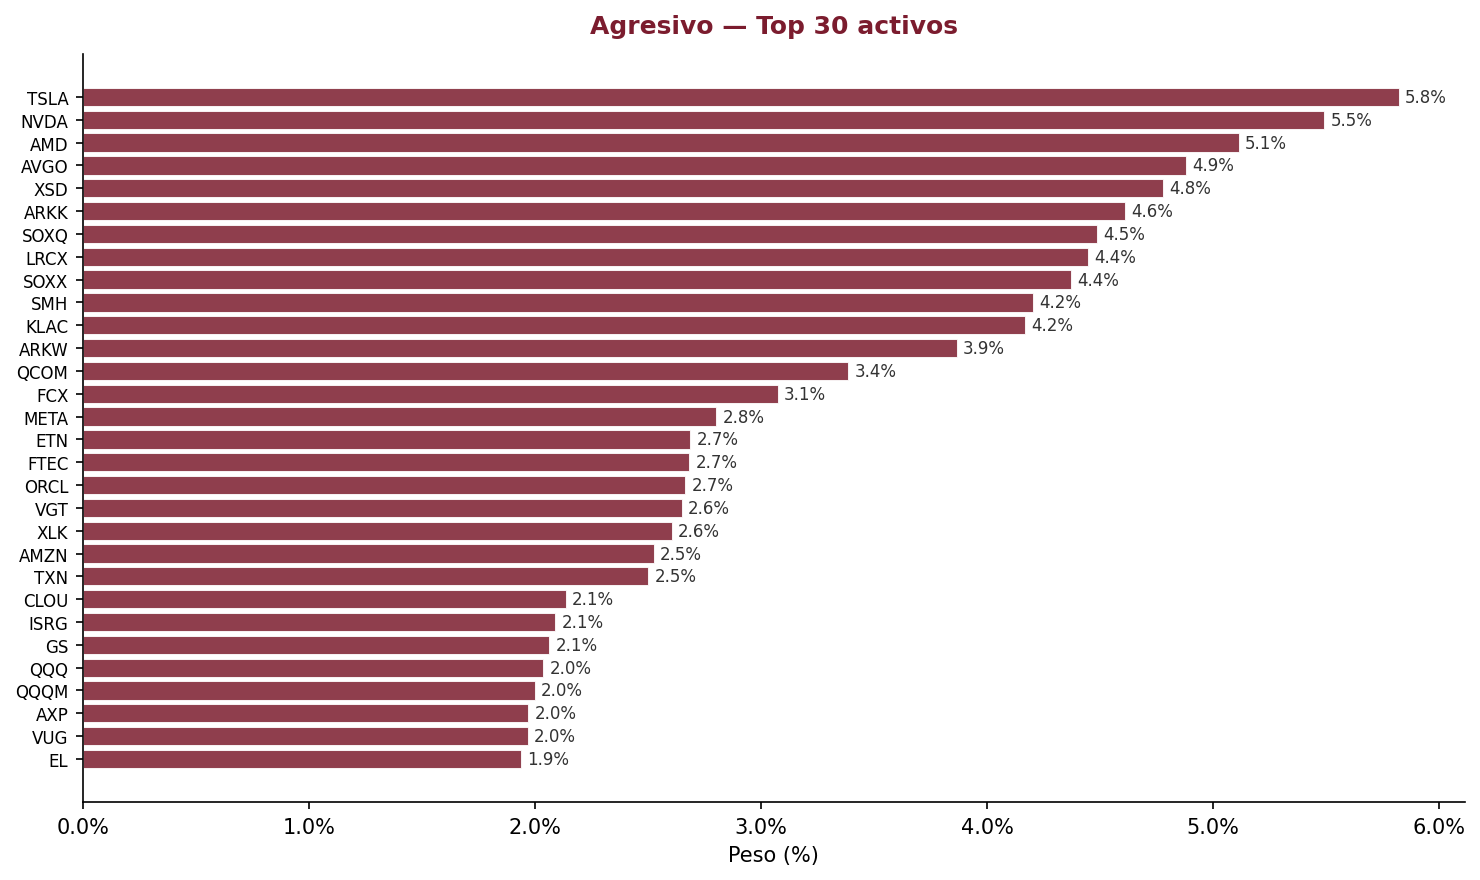
\includegraphics[width=0.85\textwidth]{../output/grafico-pesos-aggressive.png}
    \caption{Pesos de los top 30 activos en el portafolio Agresivo.}
    \label{fig:pesos_agresivo}
\end{figure}

\begin{table}[htbp]
\centering
\begin{tabular}{lrrrrrrr}
\hline
Portafolio & $NAV_{inicio}$ & $NAV_{fin}$ & $R_{total}$ & $R_{anual}$ & Vol. anual & Sharpe & Max Drawdown \\
\hline
Agresivo & 10{.}000{,}0 & 18{.}834{,}6 & 0,88 & 0,89 & 0,26 & 3,28 & -0,16 \\
\hline
\end{tabular}
\caption{Backtest Agresivo}
\label{tab:backtest-aggressive}
\end{table}
\vspace{0.5cm}
\begin{table}[htbp]
\centering
\begin{tabular}{lrrrrrr}
\hline
Símbolo & Fuente & $\beta$ & $E(R)$ & Vol. anual & Sharpe & $w$ \\
\hline
TSLA & sp500 & 2.2645 & 0.3757 & 0.6258 & 0.5364 & 0.0582 \\
NVDA & S\&P500 & 2.1748 & 0.3624 & 0.5493 & 0.5870 & 0.0549 \\
AMD & S\&P500 & 2.0717 & 0.3471 & 0.5043 & 0.6090 & 0.0511 \\
AVGO & S\&P500 & 2.0080 & 0.3377 & 0.5162 & 0.5767 & 0.0488 \\
XSD & fintual & 1.9806 & 0.3336 & 0.3893 & 0.7543 & 0.0478 \\
ARKK & fintual & 1.9344 & 0.3268 & 0.4047 & 0.7086 & 0.0461 \\
SOXQ & Fintual & 1.9017 & 0.3219 & 0.3761 & 0.7497 & 0.0449 \\
LRCX & S\&P500 & 1.8902 & 0.3202 & 0.4393 & 0.6379 & 0.0445 \\
SOXX & Fintual & 1.8694 & 0.3171 & 0.3688 & 0.7514 & 0.0437 \\
SMH & Fintual & 1.8245 & 0.3105 & 0.3652 & 0.7407 & 0.0420 \\
KLAC & S\&P500 & 1.8144 & 0.3090 & 0.4194 & 0.6413 & 0.0417 \\
ARKW & Fintual & 1.7326 & 0.2968 & 0.3625 & 0.7086 & 0.0387 \\
QCOM & S\&P500 & 1.6022 & 0.2775 & 0.3806 & 0.6241 & 0.0339 \\
FCX & S\&P500 & 1.5172 & 0.2649 & 0.4012 & 0.5606 & 0.0307 \\
META & S\&P500 & 1.4433 & 0.2540 & 0.3617 & 0.5915 & 0.0280 \\
ETN & S\&P500 & 1.4118 & 0.2493 & 0.3253 & 0.6433 & 0.0269 \\
FTEC & Fintual & 1.4108 & 0.2491 & 0.2494 & 0.8385 & 0.0268 \\
ORCL & S\&P500 & 1.4055 & 0.2484 & 0.3781 & 0.5511 & 0.0266 \\
VGT & Fintual & 1.4017 & 0.2478 & 0.2476 & 0.8391 & 0.0265 \\
XLK & Fintual & 1.3896 & 0.2460 & 0.2480 & 0.8305 & 0.0261 \\
AMZN & S\&P500 & 1.3675 & 0.2427 & 0.3136 & 0.6465 & 0.0252 \\
TXN & S\&P500 & 1.3613 & 0.2418 & 0.3175 & 0.6356 & 0.0250 \\
CLOU & Fintual & 1.2618 & 0.2271 & 0.2550 & 0.7334 & 0.0214 \\
ISRG & S\&P500 & 1.2490 & 0.2252 & 0.3067 & 0.6037 & 0.0209 \\
GS & S\&P500 & 1.2418 & 0.2241 & 0.2853 & 0.6453 & 0.0206 \\
QQQ & Fintual & 1.2350 & 0.2231 & 0.2122 & 0.8626 & 0.0204 \\
QQQM & Fintual & 1.2245 & 0.2215 & 0.2106 & 0.8620 & 0.0200 \\
AXP & S\&P500 & 1.2168 & 0.2204 & 0.2739 & 0.6585 & 0.0197 \\
VUG & Fintual & 1.2159 & 0.2203 & 0.2077 & 0.8677 & 0.0197 \\
EL & S\&P500 & 1.2081 & 0.2191 & 0.4649 & 0.3852 & 0.0194 \\
\hline
\end{tabular}
\caption{Portafolio Agresivo}
\label{tab:portafolio-aggressive}
\end{table}

\subsection{Perfil Moderado}
Funciona como una aproximación indexada general, priorizando el tope de su matriz de asignación a ETFs como ESGU, VOO e IVV.
\begin{figure}[H]
    \centering
    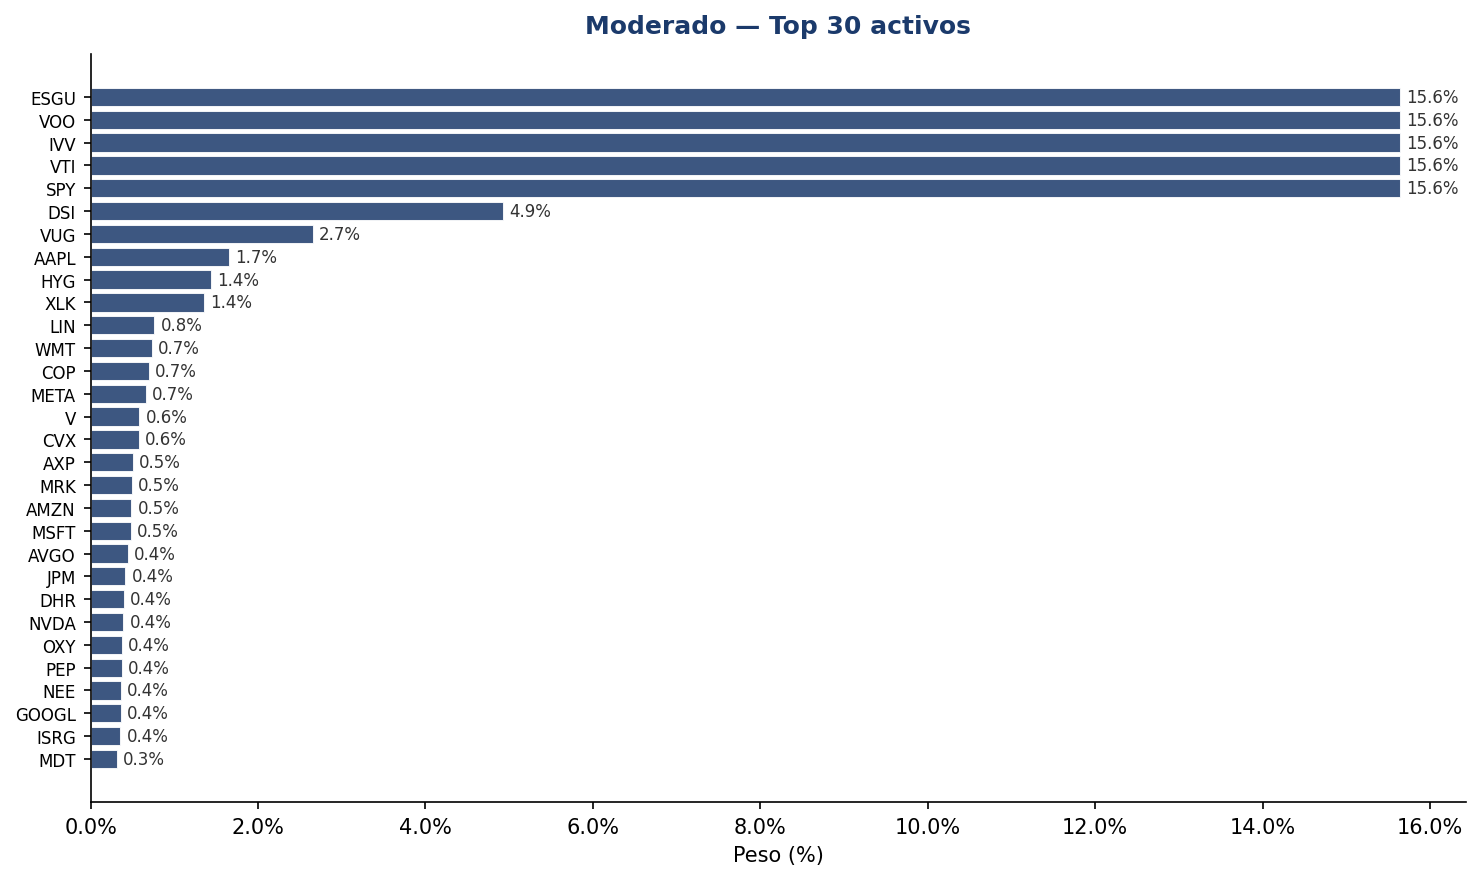
\includegraphics[width=0.85\textwidth]{../output/grafico-pesos-moderate.png}
    \caption{Pesos de los top 30 activos en el portafolio Moderado.}
    \label{fig:pesos_moderado}
\end{figure}

\begin{table}[htbp]
\centering
\begin{tabular}{lrrrrrrr}
\hline
Portafolio & $NAV_{inicio}$ & $NAV_{fin}$ & $R_{total}$ & $R_{anual}$ & Vol. anual & Sharpe & Max Drawdown \\
\hline
Moderado & 10{.}000{,}0 & 13{.}051{,}36 & 0{,}31 & 0{,}31 & 0{,}12 & 2{,}17 & -0{,}08 \\
\hline
\end{tabular}
\caption{Backtest Moderado}
\label{tab:backtest-moderate}
\end{table}
\vspace{0.5cm}
\begin{table}[htbp]
\centering
\begin{tabular}{lrrrrrr}
\hline
Símbolo & Fuente & $\beta$ & $E(R)$ & Vol. anual & Sharpe & $w$ \\
\hline
IVV & Fintual & 0.9721 & 0.1841 & 0.1594 & 0.9043 & 0.1565 \\
VTI & Fintual & 1.0039 & 0.1888 & 0.1649 & 0.9024 & 0.1565 \\
ESGU & Fintual & 0.9942 & 0.1874 & 0.1632 & 0.9033 & 0.1565 \\
VOO & Fintual & 0.9647 & 0.1830 & 0.1582 & 0.9039 & 0.1565 \\
SPY & Fintual & 1.0000 & 0.1882 & 0.1636 & 0.9060 & 0.1565 \\
DSI & Fintual & 1.0224 & 0.1916 & 0.1705 & 0.8890 & 0.0493 \\
VUG & Fintual & 1.2159 & 0.2203 & 0.2077 & 0.8677 & 0.0265 \\
AAPL & S\&P500 & 1.1567 & 0.2115 & 0.2692 & 0.6370 & 0.0165 \\
HYG & Fintual & 0.2645 & 0.0792 & 0.0595 & 0.6594 & 0.0144 \\
XLK & Fintual & 1.3896 & 0.2460 & 0.2480 & 0.8305 & 0.0136 \\
LIN & S\&P500 & 0.6061 & 0.1298 & 0.1771 & 0.5073 & 0.0076 \\
WMT & S\&P500 & 0.5503 & 0.1216 & 0.2072 & 0.3937 & 0.0073 \\
COP & S\&P500 & 0.7490 & 0.1510 & 0.2776 & 0.4000 & 0.0069 \\
META & S\&P500 & 1.4433 & 0.2540 & 0.3617 & 0.5915 & 0.0066 \\
V & S\&P500 & 0.7151 & 0.1460 & 0.1849 & 0.5733 & 0.0058 \\
CVX & S\&P500 & 0.5963 & 0.1284 & 0.2289 & 0.3862 & 0.0057 \\
AXP & S\&P500 & 1.2168 & 0.2204 & 0.2739 & 0.6585 & 0.0050 \\
MRK & S\&P500 & 0.2729 & 0.0805 & 0.2217 & 0.1825 & 0.0049 \\
AMZN & S\&P500 & 1.3675 & 0.2427 & 0.3136 & 0.6465 & 0.0049 \\
MSFT & S\&P500 & 1.0320 & 0.1930 & 0.2357 & 0.6491 & 0.0048 \\
AVGO & S\&P500 & 2.0080 & 0.3377 & 0.5162 & 0.5767 & 0.0044 \\
JPM & S\&P500 & 0.8794 & 0.1704 & 0.2341 & 0.5570 & 0.0042 \\
DHR & S\&P500 & 0.8121 & 0.1604 & 0.2570 & 0.4684 & 0.0040 \\
NVDA & S\&P500 & 2.1748 & 0.3624 & 0.5493 & 0.5870 & 0.0039 \\
OXY & S\&P500 & 0.8148 & 0.1608 & 0.2816 & 0.4289 & 0.0037 \\
PEP & S\&P500 & 0.1767 & 0.0662 & 0.1805 & 0.1451 & 0.0037 \\
NEE & S\&P500 & 0.3997 & 0.0993 & 0.2821 & 0.2101 & 0.0036 \\
GOOGL & S\&P500 & 1.1120 & 0.2049 & 0.2952 & 0.5585 & 0.0036 \\
ISRG & S\&P500 & 1.2490 & 0.2252 & 0.3067 & 0.6037 & 0.0035 \\
MDT & S\&P500 & 0.4135 & 0.1013 & 0.2010 & 0.3050 & 0.0032 \\
\hline
\end{tabular}
\caption{Portafolio Moderado}
\label{tab:portafolio-moderate}
\end{table}

\subsection{Perfil Conservador}
Refugiado en bonos y renta fija corporativa (HYG, BND, JNK).
\begin{figure}[H]
    \centering
    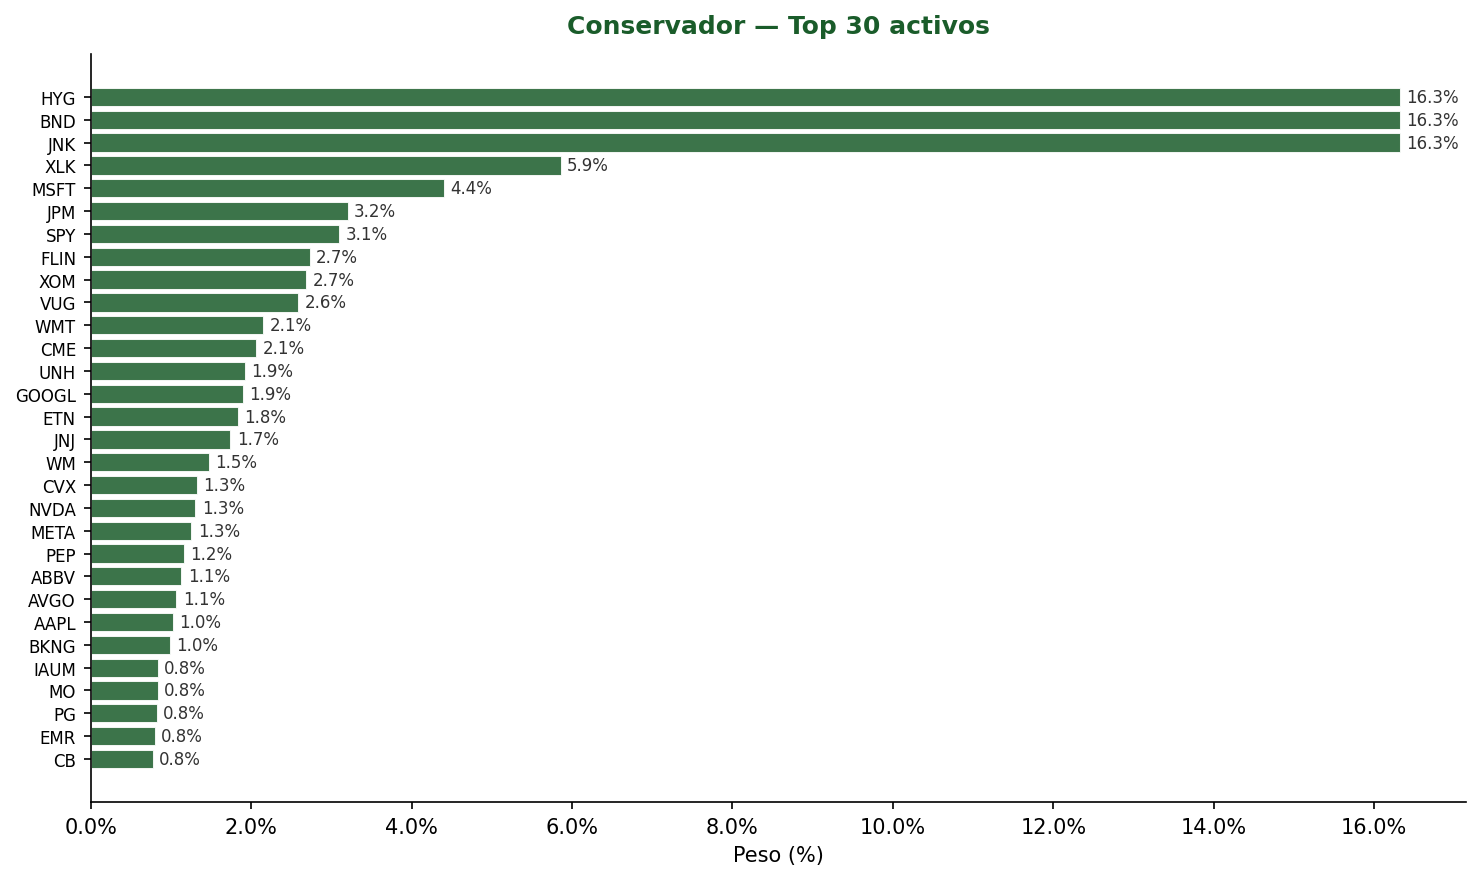
\includegraphics[width=0.85\textwidth]{../output/grafico-pesos-conservative.png}
    \caption{Pesos de los top 30 activos en el portafolio Conservador.}
    \label{fig:pesos_conservador}
\end{figure}

\begin{table}[htbp]
\centering
\begin{tabular}{lrrrrrrr}
\hline
Portafolio & $NAV_{inicio}$ & $NAV_{fin}$ & $R_{total}$ & $R_{anual}$ & Vol. anual & Sharpe & Max Drawdown \\
\hline
Conservador & 10{.}000{,}0 & 11{.}938{,}76 & 0{,}19 & 0{,}19 & 0{,}07 & 2{,}33 & -0{,}05 \\
\hline
\end{tabular}
\caption{Backtest Conservador}
\label{tab:backtest-conservative}
\end{table}
\vspace{0.5cm}
\begin{table}[htbp]
\centering
\begin{tabular}{lrrrrrr}
\hline
Símbolo & Fuente & $\beta$ & $E(R)$ & Vol. anual & Sharpe & $w$ \\
\hline
HYG & Fintual & 0.2645 & 0.0792 & 0.0595 & 0.6594 & 0.1632 \\
BND & Fintual & 0.0623 & 0.0492 & 0.0598 & 0.1543 & 0.1632 \\
JNK & Fintual & 0.2689 & 0.0799 & 0.0601 & 0.6636 & 0.1632 \\
XLK & Fintual & 1.3896 & 0.2460 & 0.2480 & 0.8305 & 0.0586 \\
MSFT & sp500 & 1.0320 & 0.1930 & 0.2357 & 0.6491 & 0.0441 \\
JPM & sp500 & 0.8794 & 0.1704 & 0.2341 & 0.5570 & 0.0320 \\
SPY & Fintual & 1.0000 & 0.1882 & 0.1636 & 0.9060 & 0.0310 \\
FLIN & Fintual & 0.4195 & 0.1022 & 0.1412 & 0.4404 & 0.0273 \\
XOM & sp500 & 0.4435 & 0.1058 & 0.2234 & 0.2943 & 0.0269 \\
VUG & Fintual & 1.2159 & 0.2203 & 0.2077 & 0.8677 & 0.0259 \\
WMT & sp500 & 0.5503 & 0.1216 & 0.2072 & 0.3937 & 0.0215 \\
CME & S\&P500 & 0.0405 & 0.0460 & 0.1728 & 0.0348 & 0.0207 \\
UNH & S\&P500 & 0.1827 & 0.0671 & 0.3070 & 0.0882 & 0.0192 \\
GOOGL & S\&P500 & 1.1120 & 0.2049 & 0.2952 & 0.5585 & 0.0190 \\
ETN & S\&P500 & 1.4118 & 0.2493 & 0.3253 & 0.6433 & 0.0184 \\
JNJ & S\&P500 & 0.0525 & 0.0478 & 0.1722 & 0.0452 & 0.0174 \\
WM & S\&P500 & 0.3110 & 0.0861 & 0.1780 & 0.2591 & 0.0148 \\
CVX & S\&P500 & 0.5963 & 0.1284 & 0.2289 & 0.3862 & 0.0133 \\
NVDA & S\&P500 & 2.1748 & 0.3624 & 0.5493 & 0.5870 & 0.0131 \\
META & S\&P500 & 1.4433 & 0.2540 & 0.3617 & 0.5915 & 0.0126 \\
PEP & S\&P500 & 0.1767 & 0.0662 & 0.1805 & 0.1451 & 0.0116 \\
ABBV & S\&P500 & 0.3364 & 0.0899 & 0.2318 & 0.2151 & 0.0113 \\
AVGO & S\&P500 & 2.0080 & 0.3377 & 0.5162 & 0.5767 & 0.0107 \\
AAPL & S\&P500 & 1.1567 & 0.2115 & 0.2692 & 0.6370 & 0.0103 \\
BKNG & S\&P500 & 1.0506 & 0.1957 & 0.2803 & 0.5556 & 0.0099 \\
IAUM & Fintual & 0.1620 & 0.0640 & 0.1466 & 0.1638 & 0.0084 \\
MO & S\&P500 & 0.1418 & 0.0610 & 0.1791 & 0.1173 & 0.0084 \\
PG & S\&P500 & 0.1528 & 0.0626 & 0.1670 & 0.1357 & 0.0082 \\
EMR & S\&P500 & 1.1387 & 0.2088 & 0.2733 & 0.6176 & 0.0080 \\
CB & S\&P500 & 0.2952 & 0.0838 & 0.1932 & 0.2265 & 0.0078 \\
\hline
\end{tabular}
\caption{Portafolio Conservador}
\label{tab:portafolio-conservative}
\end{table}

\end{document}
